
\section[Statistics]{Summary and statistical interpretation of the results}
\label{sect:stat}

To interpret the results, we first recapitulate a little of assumptions and the consequent numbers.
In this analysis, we examine the data in three different channels.
These channels include \tauTau, \muTau and \eTau.
The signal region for the \muTau and \eTau channels is defined in one bin, which is $\mttwo > 90$ and $\tauMT > 200$ .
Due to the sensitivity of \tauTau channel to the signal, we look at the data in two different bins.
The first bin is $\mttwo > 90$ and the second one is $40 < \mttwo < 90$ and $\SumMT > 250$.
We eventually combine all four bins to utilize more information from the observed and the predicted distributions.


Backgrounds are taken into account in two categories, including Monte-Carlo-Driven (MCD) and Data-Driven (DD).
However, due to the method of background estimation in the \tauTau channel, \binone and \bintwo of this channel have one more category called W-jets (W).
As a summary of results, the background yields and systematic uncertainities are listed in Table \ref{tbl:yieldSysSummary}.
As seen in the Table, the overall background yields of all categories, for the \tauTau channel \binone and \bintwo and \eTau and \muTau channels are  1.5, 3.01, 2.7 and 1.06 respectively (sum of three first rows of Table \ref{tbl:yieldSysSummary}).
MCD backgrounds are feed to the package as a Gamma distribution with the corresponding statistical weights for each bin.
Furthermore, 25\% systematic uncertainity on MCD backgrounds is also considered.
All systematics are taken through LogNormal distributions.
Systematic uncertainities for each bin of DD backgrounds are 111\%, 215\%, 50\% and 69\% respectively.  
W backgronds have 37\% and 45\% systematic uncertainity for the first and second bins respectively.
And finally, 20\% systematic uncertainity on signal yields is considered. 


\begin{table}[h]
\begin{center}
%\begin{tiny}
\begin{tabular}{l|l|l|l|l}
\hline
\hline
	& \tauTau\binone & \tauTau\bintwo & \eTau\binone & \muTau\binone \\
\hline
\hline
MCD (yield) & 0.75 & 1.56 & 0.2 & 0.45 \\
DD (yield) & 0.09 & 0.65 & 2.5 & 0.61 \\
W (yield) & 0.66	 & 0.8 & - & - \\
%\hline				
%MCD (sta.) & 81x0.00926 &  4x0.39 & 800x0.00025 & 8x0.0563 \\
\hline
MCD (sys.) & 25\%	 & 25\% & 25\% & 25\% \\
DD (sys.) & 111\% & 	215\% & 50\% & 69\% \\
W (sys.) & 37\% & 45\% & - & - \\
\hline
\hline
\end{tabular}
\caption{Summary of background yields and corresponding systematic uncertainities.}
\label{tbl:yieldSysSummary}
%\end{tiny}
\end{center}
\end{table}


If no excess of data over the background prediction is observed, 
we close our study with setting upper limits on the testing signals.
This is conducted using a modified frequentist approach, namely CLs method \cite{read:CLs}.
In this method, the test statistic $q_\mu$ 
%\cite{cowan:asymptoticCLs} 
is a function of the profile likelihood-ratio,

\begin{align}
q_\mu = -2 \ln \frac{\mathcal{L}(data ;\, b + \mu s)}{\mathcal{L}(data ;\, b + \hat{\mu} s)},
\end{align}

where $\hat\mu$ is the \textit{signal strength modifier} $\mu$ at the maximum point of the likelihood $\mathcal{L}$.
Then CLs is given by the following probability-ratio,

\begin{align}
CL_s = \frac{p(q_\mu \geq q_\mu^{obs} | b + \mu s )}{p(q_\mu \geq q_\mu^{obs} | b)}.
\end{align}
 
We compute CLs using a software package provided by the CMS Higgs PAG \cite{higgspag:software}.
After incorporating systematic uncertainties, an observed CLs smaller than 0.05 for a signal strength of $\mu = 1$, excludes the given signal at $95\%$ CL. Indeed, the package determines which signal strength $\mu$ excludes the testing signal at $95\%$ CL. Therefore all resulting $\mu \leq 1$ define the excluded region in the parameter space of the given signal. 

%To investigate the exclusion power of our research, we study the topology of direct stau pair production and the \PSGcpDo\PSGcmDo production in Simplified Models \cite{alves:sms}. 
%This research deal with tau family decay of charginoes including 
%$ \chione \rightarrow \sTau + \nu ~~\mathrm{and}~~  \chione \rightarrow \sNu_{\tau} + \tau $.
%As discussed in Section \ref{sect:introduction}, the final state is full of $\tau$ and $ \sTau \rightarrow \tau + \PSGczDo  $.
%Hence many channels could be define, due to decays of tau to electrons, muons and hadrons.    

Panels represented in Figure \ref{fig:limit_bins} show the impact of each bin on the combined result, represented by the final exclusion limit shown in Figure \ref{fig:limit_final}. The top-left panel of Figure \ref{fig:limit_bins} shows the expected exclusion region in the plane of $m_{\chione}-m_{\PSGczDo}$
calculated by the simulated samples in the first bin of \tauTau channel. The top-right panel in Figure \ref{fig:limit_bins} is produced by using both bins of \tauTau channel.
As seen, the inclusion of \bintwo in the \tauTau channel causes a little expansion of the exclusion limit toward the left side (low mass $\chione$).
Two bottom panels of Figure \ref{fig:limit_bins} show the expected exclusion limit when \eTau (left) and \muTau (right) channels are 
added to the \tauTau channel.  As seen, these channels individually improves the limit on the right side of plane (high mass $\chione$).


%%%%%%%%%%
\begin{linenomath}
\begin{figure}[h]
\centering
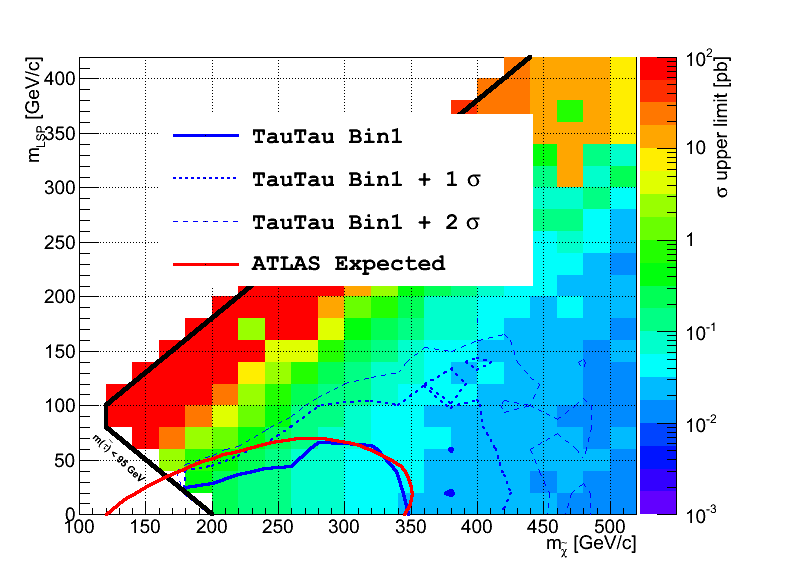
\includegraphics[width=0.49\textwidth,keepaspectratio=true]{StatisticsFig/RealisticsSystematics/Exclusion_TauTauBin1Rel.png}
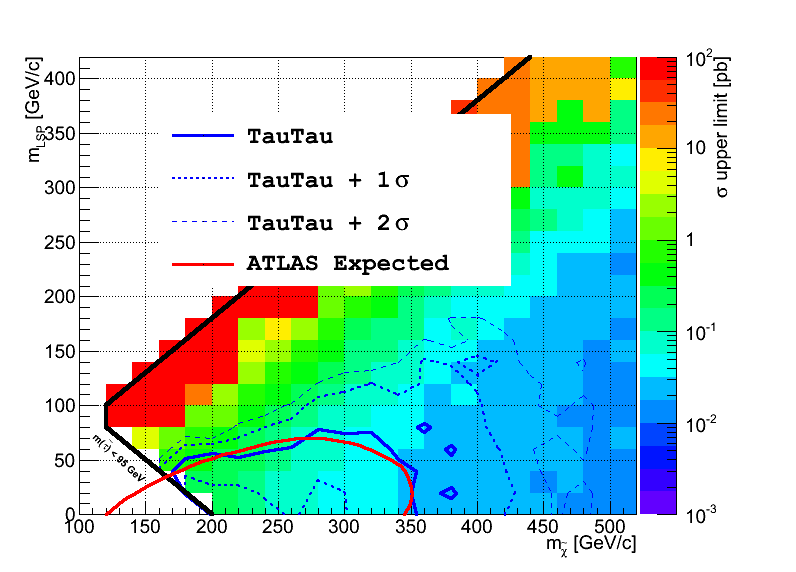
\includegraphics[width=0.49\textwidth,keepaspectratio=true]{StatisticsFig/RealisticsSystematics/Exclusion_TauTauBin1Rel_Bin2.png}
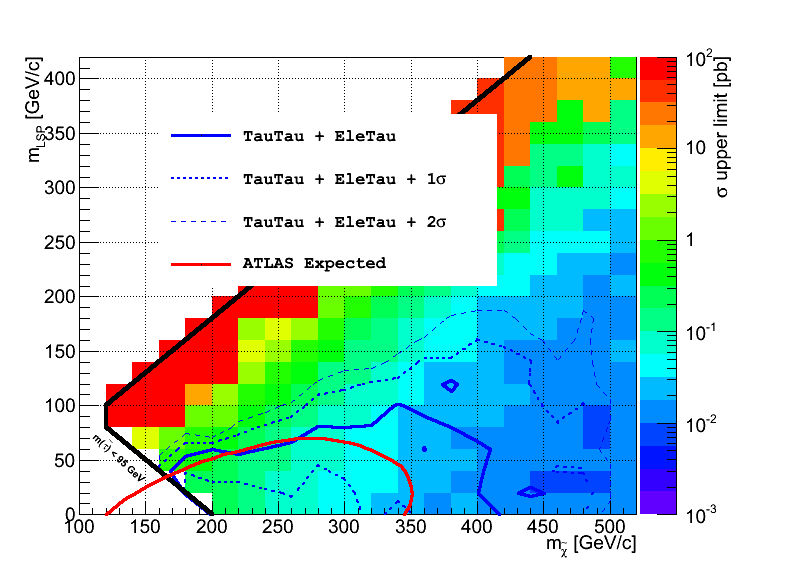
\includegraphics[width=0.49\textwidth,keepaspectratio=true]{StatisticsFig/RealisticsSystematics/Exclusion4Bins_MuTauExcl.png}
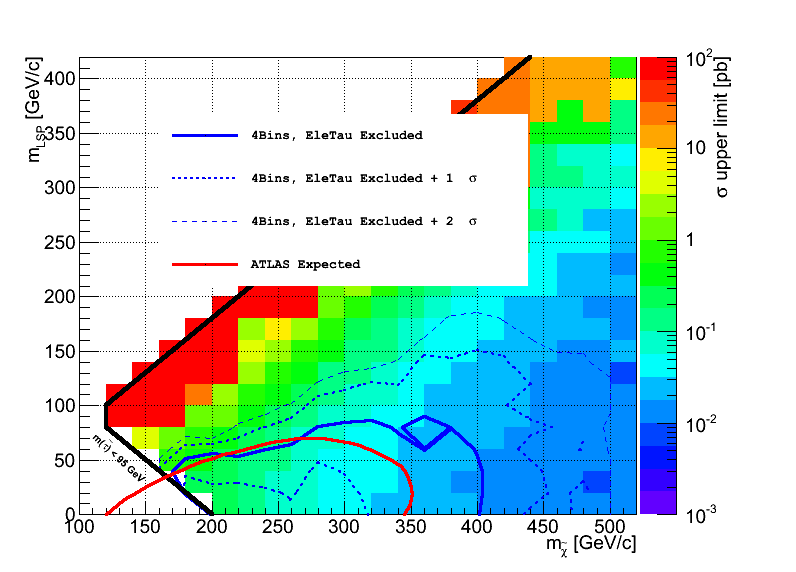
\includegraphics[width=0.49\textwidth,keepaspectratio=true]{StatisticsFig/RealisticsSystematics/Exclusion4Bins_EleTauExcl.png}
\caption{These figures show the impact of each bin on the final combination. 
The top panels are related to the \tauTau channel including the \binone alone (left) and combination of \binone and \bintwo (right).
The bottom ones show the expected exclusion limit when \eTau (left) and \muTau (right) channels are included in the \tauTau channel.
}
\label{fig:limit_bins}
\end{figure}
\end{linenomath}
%%%%%%%%%%


Figure \ref{fig:limit_final} shows the expected upper limit on the cross section of the chargino pair production in terms of Simplified Models \cite{alves:sms}. 
Calculation of the expected exclusion limit shows that the research has potential to exclude 
a sizable region of the phase space, surrounded by the lines of $m_{\chione} = 500\GeV$ and $m_{\PSGczDo} = 150\GeV$ with 
the total dataset of 2012.
The Red curve represents the expected reach by ATLAS %\cite{cutandcountAN}
search. As the figure shows, our analysis (the blue solid curve) is well above the ATLAS result in the $m_{\chione}-m_{\PSGczDo}$ plane.


%%%%%%%%%%
\begin{linenomath}
\begin{figure}[h]
\centering
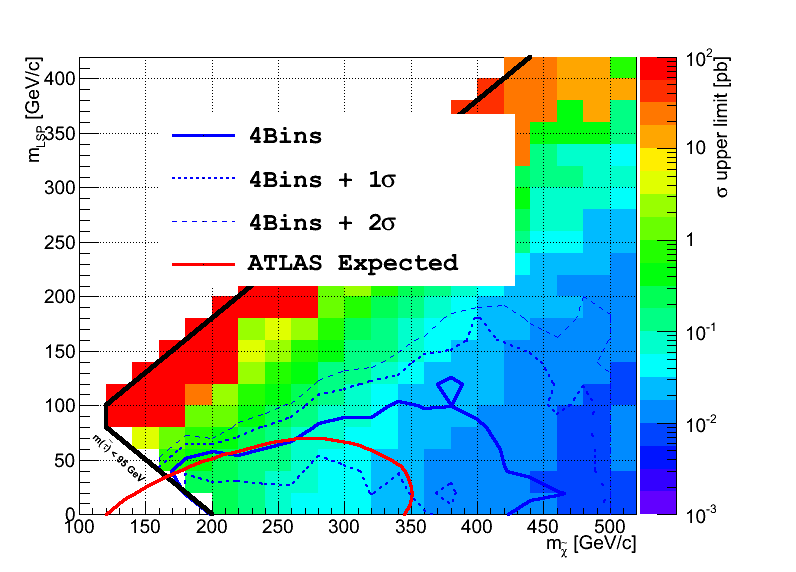
\includegraphics[width=0.7\textwidth,keepaspectratio=true]{StatisticsFig/RealisticsSystematics/Exclusion4Bins.png}
\caption{Expected exclusion power in terms of Simplified Models
with the total dataset of 2012. 
%Backgrounds are predicted using Monte-Carlo simulations and a rough estimate of systematic uncertainties equal $10\%$ is taken into account.
}
\label{fig:limit_final}
\end{figure}
\end{linenomath}
%%%%%%%%%%
